\chapter{Postup}
\label{5-postup}

\section{Aktualizace pluginu do verze 1.0.0}
Po dokončení pluginu v předmětu Free Software GIS měl plugin veškerou základní 
funkcionalitu, kterou měl mít. Tou bylo načítání GTFS ZIP souboru do QGISu,
rozbalení ZIP souboru, načtení CSV souborů do geodatabázového kontajneru GeoPackage,
vytvoření vektorových vrstev pro soubory \textit{stops.txt} a \textit{shapes.txt},
obarvení vektorové vrty \textit{shapes.txt} a vložení do CSV souborů a vrstev do
\textit{layer tree}.
% vysvětlit layer tree, GeoPackage??

Avšak pro uvedení do "ostrého" provozu musel být plugin více uživatelsky přívětivější.
Proto byl veškerý proces přesunut na pozadí, aby celý QGIS program "nezamrzal" a
mohla se při jeho výpočtech provádět i jiné akce. To se provedlo díky python třídě \textit{QgsTask}
a jejím metodám, které byly zděděny z této třídy. \cite{QgsTask}
% dát sem i ukázku kódu? 

Pro zobrazování procesu během výpočtu byla použita třída \textit{QProgressBar} a její metody.
Zobrazení postupu bylo implementováno do lišty zpráv QGISu spolu s chybovými hláškami.

\begin{figure}[H] \centering
    
\includegraphics[width=400pt]{./pictures/loading.png}
    \caption[ProgressBar]{ProgressBar v liště QGISu}
	\label{fig:ProgressBar v liště QGISu}              
\end{figure}     

% možná přidat code refactorization

\section{Postup 1 - pomocí nástrojů QGIS}

Pro použití QGIS nástrojů v pythoním skriptu je potřeba importovat modul \textit{processing},
který má funkci \textit{run}, do které se vkládají dva parametry. První parametr je ID nástroje
ve formě \textit{stringu} a druhý je \textit{slovník} vstupních parametrů. Vstupní parametry se lze dozvědět
z QGIS dokumentace. \cite{QGIS_docs}

\subsection{Hrubý tvar tarifních pásem}

GTFS obsahuje povinný CSV soubor \textit{stops.txt}. Tento soubor obsahuje mimo
jiných polí také pole \textit{zone\_id}, které bylo při tvorbě tarifních pásem klíčové. 
Pole \textit{zone\_id} má datový typ \textit{string} a znamená, ve kterém tarifním
pásmu daná zastávka leží. Verze GTFS Loaderu 1.0.0 soubor \textit{stops.txt} převádí do vektorové vrstvy
ve formě bodů. Z této bodové vrstvy byla vytvořena vektorová vrstva Voroného 
diagramů nástrojem \textit{Voroného polygony} v programu QGIS. 

Vstupem do tohoto nástroje je vektorová vrstva stops a výstupem jsou právě Voroného polygony.

\begin{figure}[H] \centering
    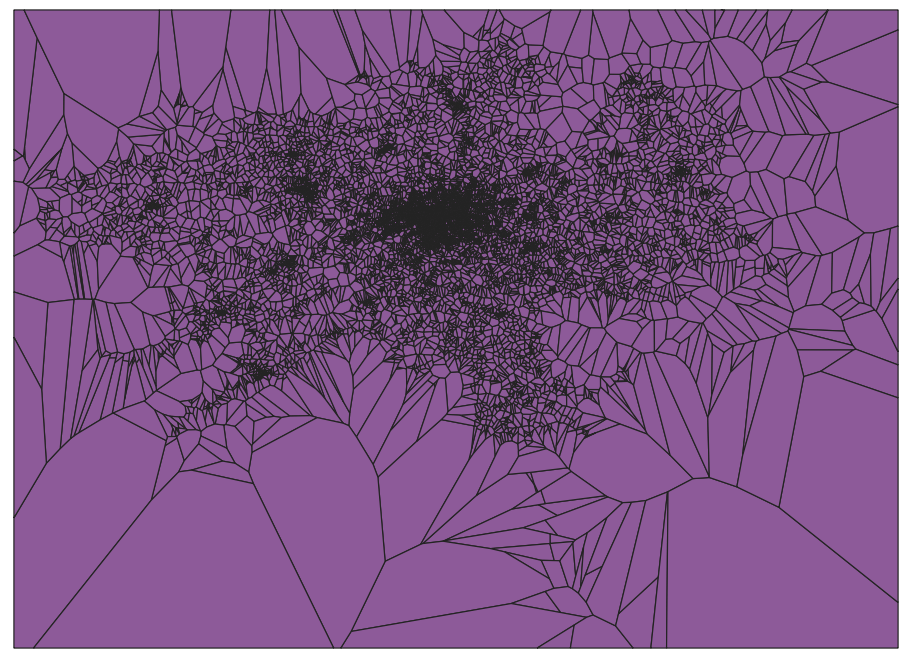
\includegraphics[width=400pt]{./pictures/voronoi-stops.png}
    \caption[Voroného polygony pro všechny zastávky]{Voroného polygony pro všechny zastávky}
	\label{fig:voronoi-stops}              
\end{figure}
  
Pro každé tarifní pásmo byly vybrány zastávky pomocí třídy \textit{QgsVectorLayer}
a její metody \textit{selectByExpression}, která vybírá prvky podle zadaného výrazu ve formě \textit{string}.
Znění zadaného výrazu je následující:

%zjistit, jak lépe přidat části kódu
\textit{zone\_id in "tarifní pásmo" and location\_type = 0}

V zadávaném výrazu figuruje taktéž údaj o poli \textit{location\_type}, což je typ lokace. 
Hodnota nuly (nebo prázdná hodnota) je právě lokace zastávky. 
Třída \textit{QgsVectorLayer} představuje zároveň vektorovou vrstvu, která spravuje
vektorové datové sady a která může být považována jako vstup do nástroje QGIS. % tim chci rict, ze do vstupu nemuze jit string, tzn pouha cesta k vrstve

Pro vybrané zástavky bylo potřeba vybrat ty Voroného polygony, které svou
pozicí dané zastávky protínaly. To bylo provedeno nástrojem \textit{Select by location},
do kterého vstupovala vrstva vybraných zastávek a vrstva Voroného polygonů. Výsledkem tohoto nástroje byla
vektorová vrstva vybraných Voroného polygonů. Jako příklad v obrázku zde budu uvádět tarifní pásmo 2.

\begin{figure}[H] \centering
    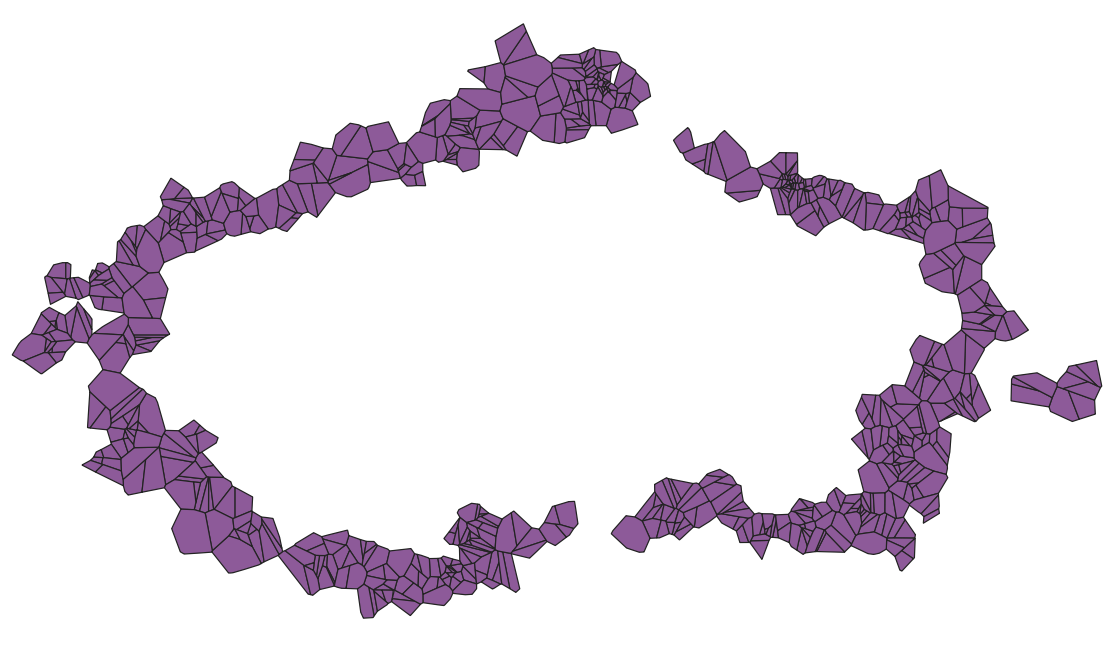
\includegraphics[width=400pt]{./pictures/voronoi-selected.png}
    \caption[Vybrané Voroného polygony pro pásmo 2]{Vybrané Voroného polygony pro pásmo 2}
	\label{fig:voronoi-selected}              
\end{figure}

Tyto polygony byly následně nástrojem \textit{Dissolve} spojeny do jednoho společného polygonu.
Vstupem tohoto nástroje byl výstup nástroje \textit{Select by location} a výstupem byl polygon
s jednou geometrií. 

\begin{figure}[H] \centering
    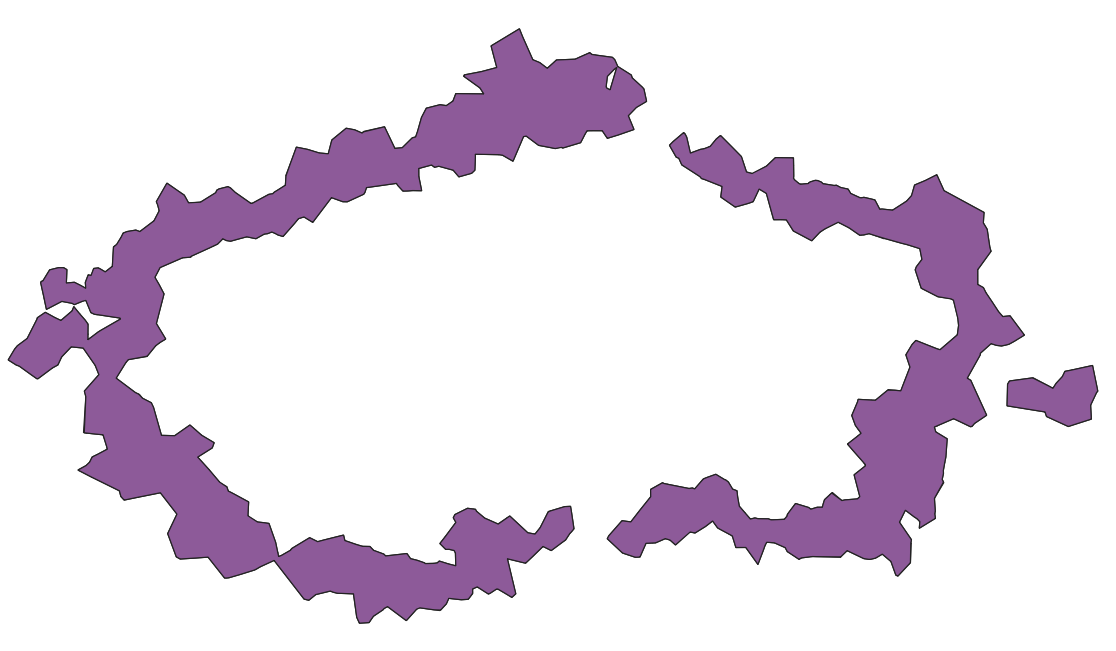
\includegraphics[width=400pt]{./pictures/dissolve.png}
    \caption[Výsledek nástroje Dissolve pro pásmo 2]{Výsledek nástroje Dissolve pro pásmo 2}
	\label{fig:dissolve}              
\end{figure} 

Znázornění tohoto postupu je zobrazeno zde v obrázku \ref{fig:postup-voronoi-P0B}. Toto zobrazení bylo provedeno v Grafickém modeláři
a ukazuje postup pro tarifní pásma P, 0 a B. V následujícím obrázku je \ref{fig:postup-voronoi-1az9} zobrazen postup tarifní pásma 1 až 9.

\begin{figure}[H] \centering
    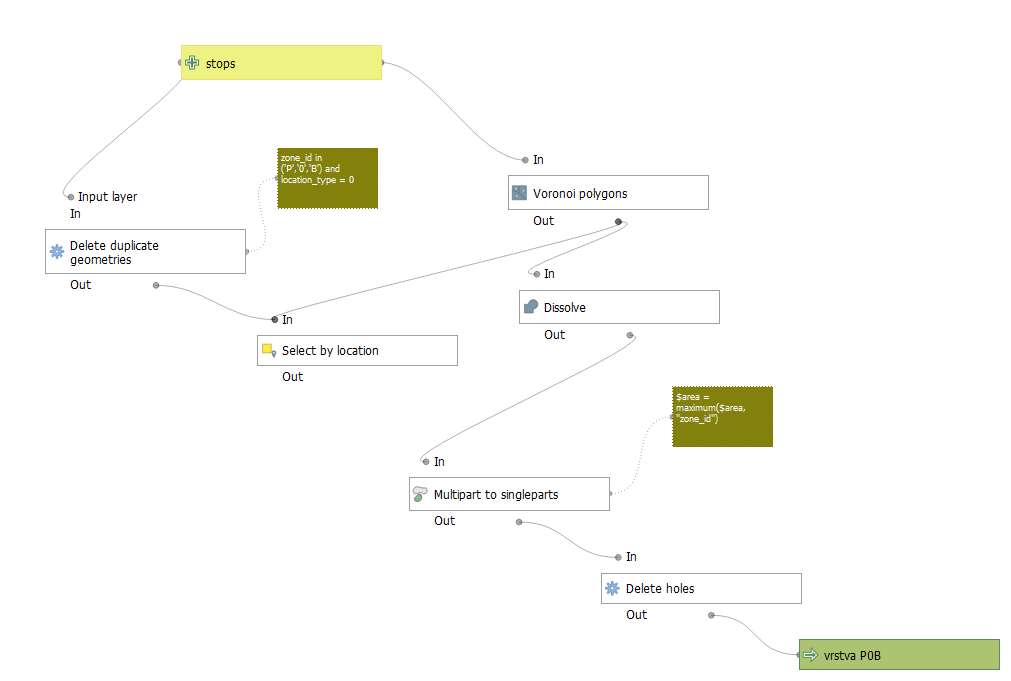
\includegraphics[width=400pt]{./pictures/postup-voronoi-P0B.png}
    \caption[Postup pro tarifní pásma P, 0 a B]{Postup pro tarifní pásma P, 0 a B}
	\label{fig:postup-voronoi-P0B}              
\end{figure}

\begin{figure}[H] \centering
    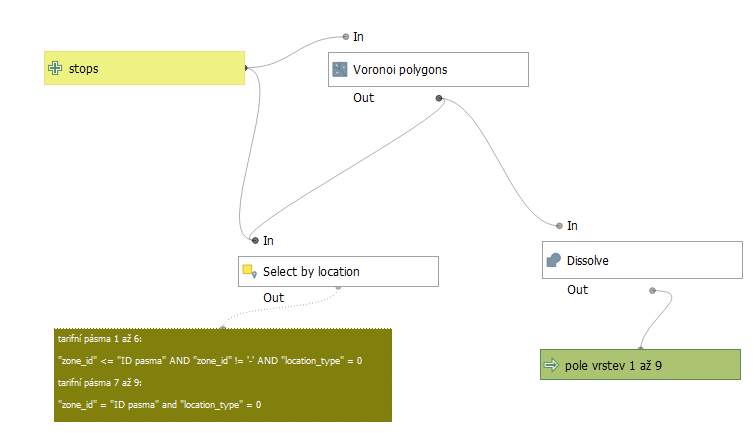
\includegraphics[width=400pt]{./pictures/postup-voronoi-1az9.png}
    \caption[Postup pro tarifní pásma 1 až 9]{Postup pro tarifní pásma 1 až 9}
	\label{fig:postup-voronoi-1az9}              
\end{figure}

\subsection{Vyhlazení tvaru tarifních pásem}

Ze spojených polygonů byla poté vygenerována vektorová vrstva bodů nástrojem
\textit{Extract vertices}, která představovala vrcholy spojených polygonů. Pro tuto vrstvu
bylo vstupem výstup nástroje \textit{Dissolve} a výstupem byl vektorová vrstva bodů 
doplněná o pole (mimo původních polí z vektorové vrstvy \textit{stops}) jako \textit{vertex\_index,
vertex\_part, vertex\_part\_ring, distance} a \textit{angle}.
Hodnoty těchto polí avšak nebyly využity v dalším výpočtu.

\begin{figure}[H] \centering
    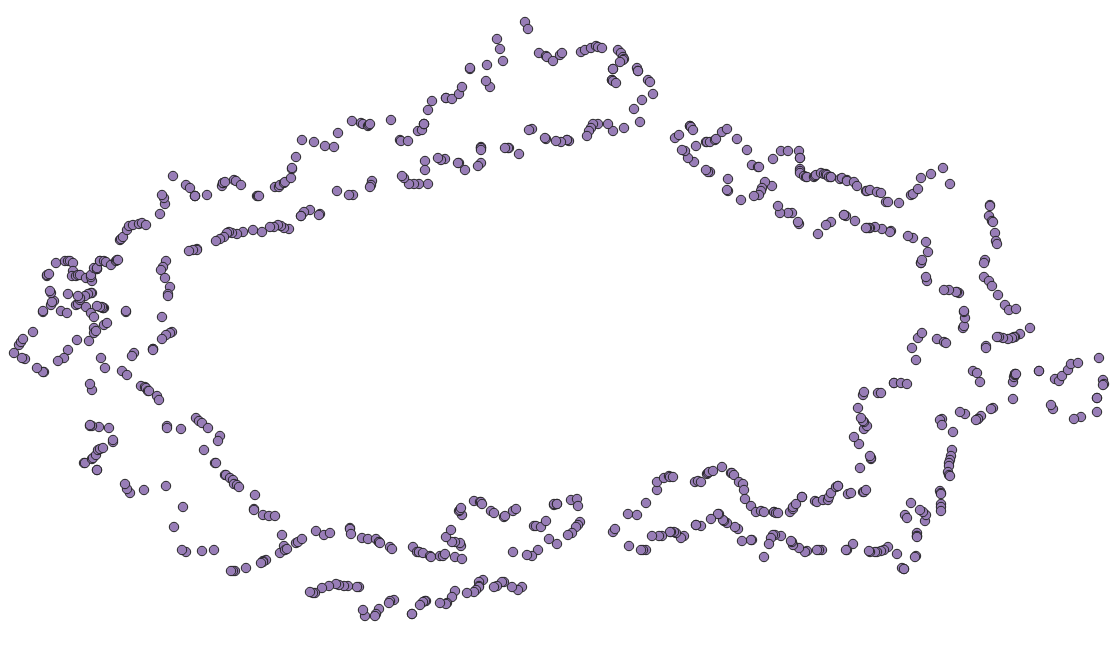
\includegraphics[width=400pt]{./pictures/vertices.png}
    \caption[Výsledek nástroje Extract vertices pro pásmo 2]{Výsledek nástroje Extract vertices pro pásmo 2}
	\label{fig:vertices}              
\end{figure} 

% ------- toto se nejspíš bude předělávat, jiná metoda řešení zastávek na hranici -------
Dále byly s pomocí třídy \textit{QgsVectorLayer} a její metody \textit{selectByExpression} vybrány 
z původní vektorové vrstvy \textit{stops} ty zastávky, které obsahovaly v poli \textit{zone\_id}
hodnotu tarifního pásma 1,2 nebo 2,3. Takové zastávky ležely na hranici pásma a polygon tarifního pásma
měl skrz ně vézt hranici. Z vybraných zastávek byla vytvořena vlastní vektorová vrstva. 
% ------- toto se nejspíš bude předělávat, jiná metoda řešení zastávek na hranici -------

Následně byly spojeny vektorové vrstvy hraniční zastávek, zastávek uvnitř tarifního pásma 2 a
bodů z výstupu nástroje \textit{Extract vertices} nástrojem \textit{Merge vector layers}.
Tyto tři zmiňované vektorové vrstvy byly vstupem do tohoto nástroje a výstupem byla 
vektorová vrstva spojených bodů. 

\begin{figure}[H] \centering
    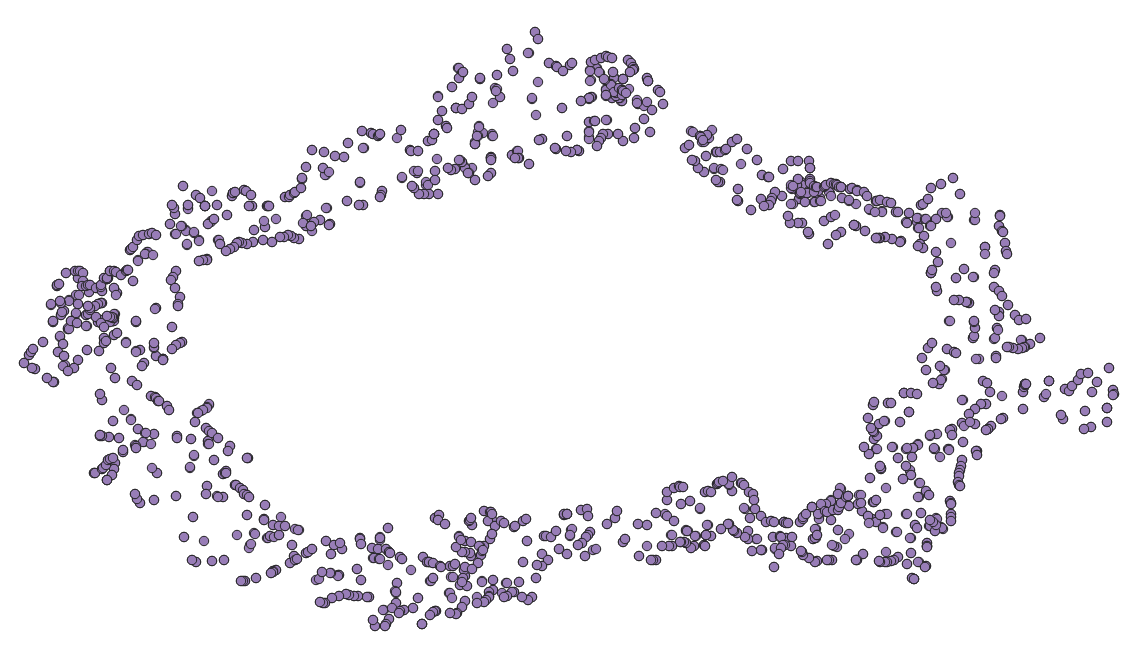
\includegraphics[width=400pt]{./pictures/merged.png}
    \caption[Spojené body třech vektorových vrstev pro pásmo 2]{Spojené body třech vektorových vrstev pro pásmo 2}
	\label{fig:merged}              
\end{figure} 

% Definice konkávní obálky 
Ze spojených bodů byla vytvořena konkávní obálka. To bylo provedeno nástrojem Concave hull (alpha shapes),
který počítá konkávní obálku z vstupních bodů. Vstupem tedy byla vrstva spojených bodů, což byl první parametr
nástroje. Dalším parametrem byl \textit{Práh (Threshold)} s datovým typem \textit{čísla}, který byl volen od 0 do 1,
kdy 0 znamenala maximum konkávní obálky a 1 konvexní obálky. Po několika testovacích spuštění byla 
určena hodnota 0,09 jako nejlepší hodnotou pro tvorbu tarifních pásem. Dalším parametrem bylo \textit{Povolení děr (Allow holes)} 
s datovým typem \textit{boolean}, který byl nastaven na \textit{False}.
Posledním parametrem bylo Rozdělit vícedílnou geometrii na jednotlivé části (Split multipart geometry 
into singlepart geometries) taktéž s datovým typem \textit{boolean}, který byl nastaven na \textit{True}.  
Výstupem byla polygonová vrstva konkávní obálky. 

\begin{figure}[H] \centering
    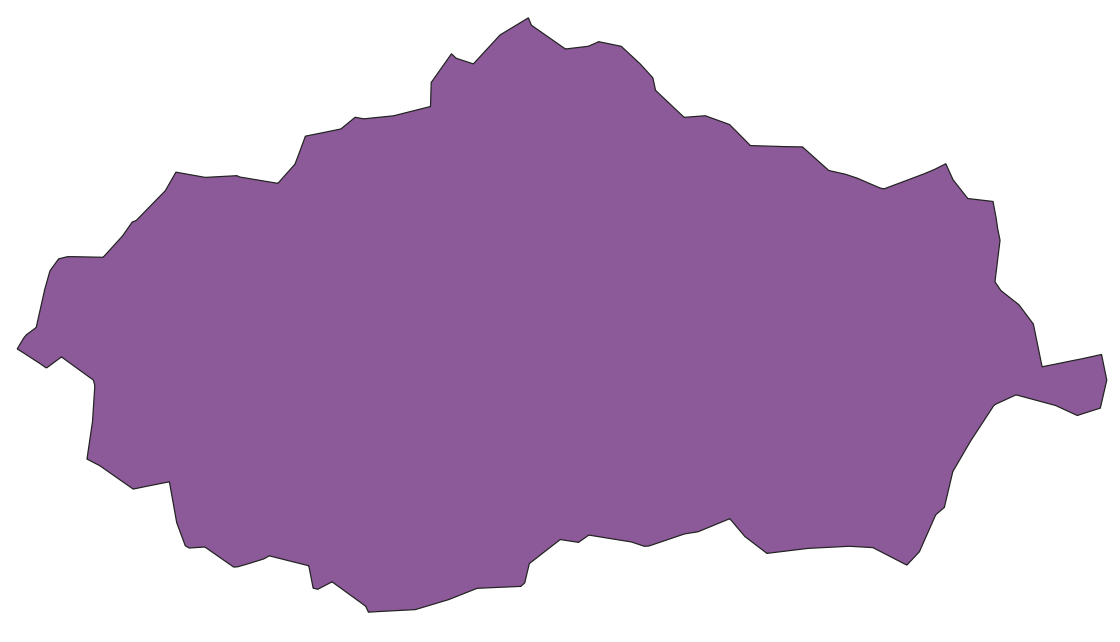
\includegraphics[width=400pt]{./pictures/concaveHull.png}
    \caption[Konkávní obálka pro pásmo 2]{Konkávní obálka pro pásmo 2}
	\label{fig:concaveHull}              
\end{figure} 

Z konkávní obálky byla pomocí nástroje Simplify "zjednodušena" geometrie polygonové vrstvy. Tento nástroj
využívá tři druhy zjednodušení vektorové vrstvy: založené na vzdálenosti (algoritmus „Douglas-Peucker“),
založené na ploše (algoritmus „Visvalingam“) a přichytávání geometrií k mřížce.
Pro můj postup byl zvolen první volba zjednodušení, pomocí algoritmu „Douglas-Peucker“.

Algoritmus „Douglas-Peucker“ na rozdíl od ostatních algoritmů neodstraňuje vrcholy nesplňující 
geometrickou podmínku, ale přidává do ní postupně kritické body, které podmínku splnují.
Tento algoritmus je jeden z nejlepších generalizacních algoritmů a je velmi často
implementován v GIS software. \cite{bayer-douglas}

\begin{figure}[H] \centering
    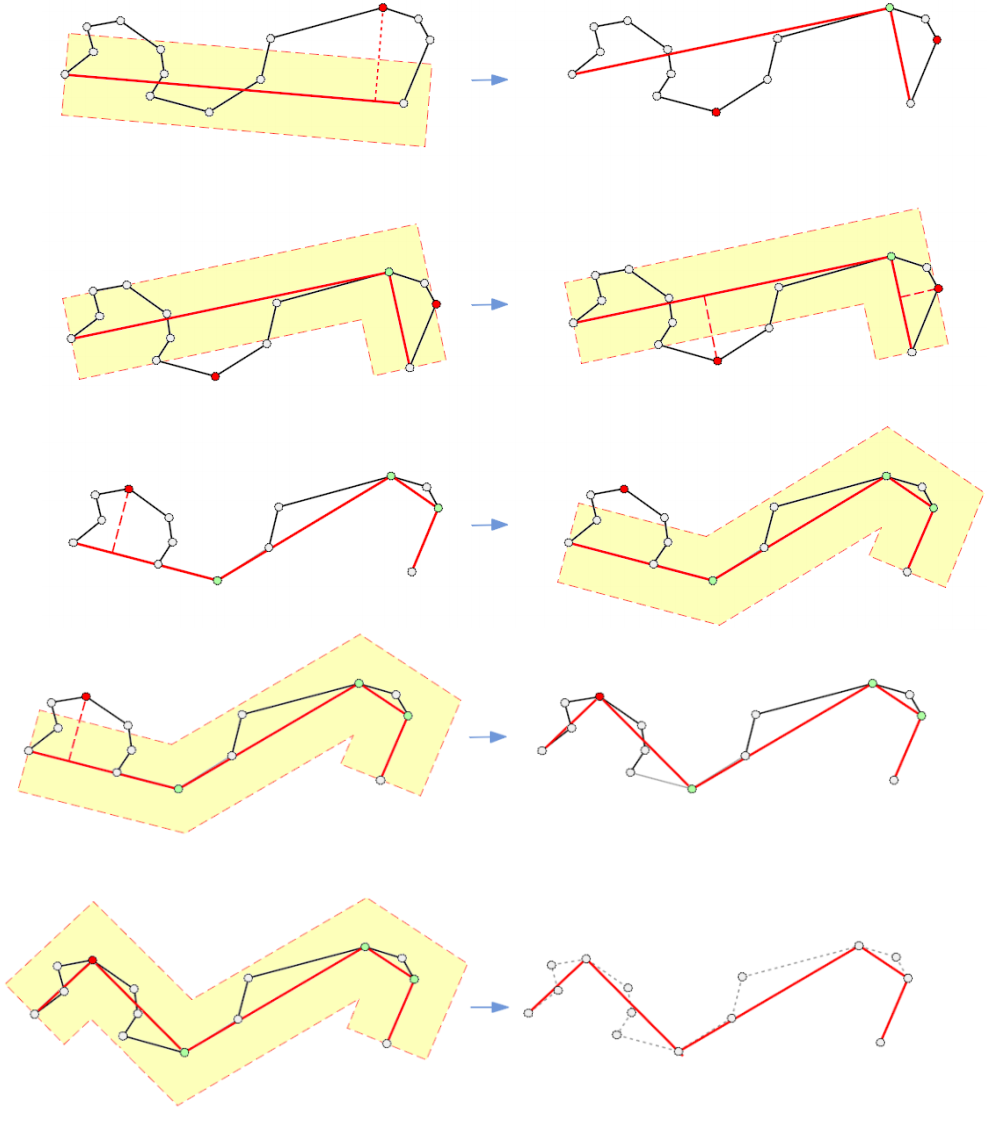
\includegraphics[width=400pt]{./pictures/douglas.png}
    \caption[Znázornění algoritmu „Douglas-Peucker“]{Znázornění algoritmu „Douglas-Peucker“ \cite{bayer-douglas}}
	\label{fig:douglas}              
\end{figure} 

Do nástroje Simplify byl vstupem výsledek nástroje Concave hull (alpha shapes), parametrem byl výběr algoritmu 
a nastavení hodnoty tolerance vzdálenosti. Výstupem byla polygonová vektorová vrstva.

\begin{figure}[H] \centering
    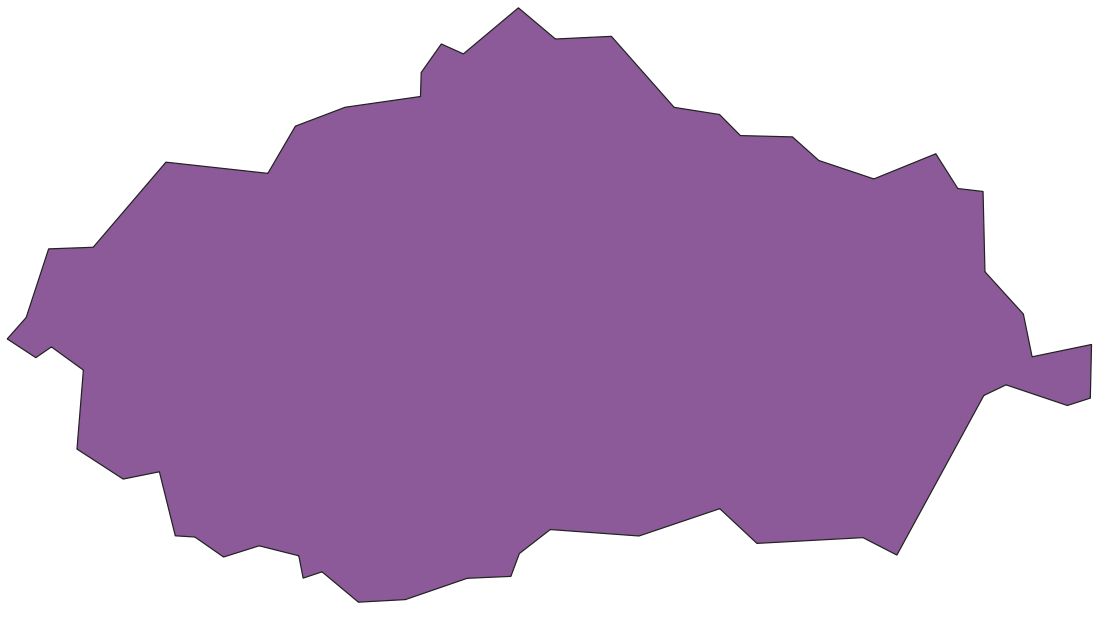
\includegraphics[width=400pt]{./pictures/simplify.png}
    \caption[Výsledek nástroje Simplify pro pásmo 2]{Výsledek nástroje Simplify pro pásmo 2}
	\label{fig:simplify}                                
\end{figure}

Výstup nástroje Simplify byl vstupem do nástroje Smooth. Tento nástroj vyhlazuje geometrie
liniové nebo polygonové vrstvy pomocí Chaikinova algoritmu.

Chaikin využil fixních poměrů na odříznutí rohů, takže byly všechny rozřezány stejně. 
Při matematickém zápisu postupuje Chaikinova metoda následovně: Dostaneme kontrolní polygon 
\textit{\{P\textsubscript{0}, P\textsubscript{1}, ..., P\textsubscript{n}\}},
tento kontrolní polygon vylepšíme vygenerováním nové posloupnosti řídicích bodů 
\[ \{Q_0, R_0, Q_1, R_1, ...,  Q_{n−1}, R_{n−1}\} \]                                    
kde každá nová dvojice bodů Q\textsubscript{i}, R\textsubscript{i} je třeba brát v poměru \(\frac{1}{4}\)
a \(\frac{3}{4}\) mezi koncovými body segmentu čáry \(\overline{P\textsubscript{i}P\textsubscript{i+1}}\).
\[Q_i = \frac{3}{4}P_i + \frac{1}{4}P_{i+1}\]
\[R_i = \frac{1}{4}P_i + \frac{3}{4}P_{i+1}\]
Tyto 2 nové body lze považovat za nový řídicí polygon - vylepšení původního řídicího polygonu. \cite{chaikin} 

U nástroje Smooth byly zvoleny tři parametry - počet iterací, offset a maximální úhel.
Počet iterací znamená, kolik vyhlazovacích iterací bude použito pro každou geometrii.
Hodnota počtu iterací byla nastavena na 10, což byla maximální volitelná hodnota (pro co nevětší hladkost).
Parametr offset znamená, jak "těsně" vyhlazené geometrie sledují původní geometrie.
Zde byla ponechána výchozí hodnota 0,25. A poslední parametr maximálního úhlu lze použít
k zabránění vyhlazení uzlů s velkými úhly. Zde byla také ponechána výchozí hodnota 180°.
Výstupem nástroje byla polygonová vektorová vrstva.

\begin{figure}[H] \centering
    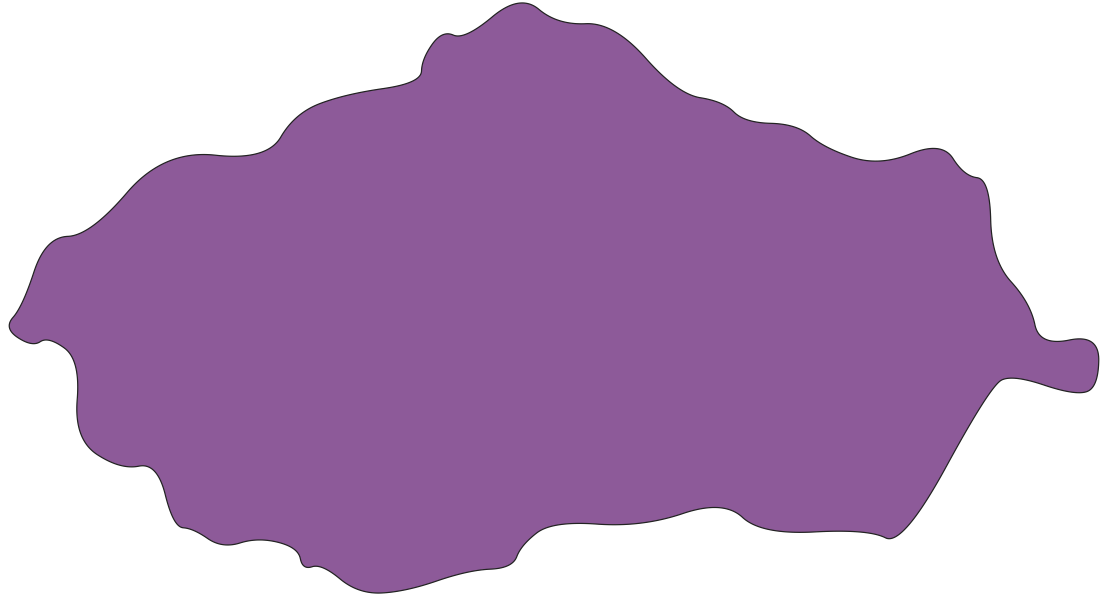
\includegraphics[width=400pt]{./pictures/smooth.png}
    \caption[Výsledek nástroje Smooth pro pásmo 2]{Výsledek nástroje Smooth pro pásmo 2}
	\label{fig:smooth}                                
\end{figure}

Zde je souhrně zobrazen postup této části na obrázku \ref{fig:postup-smooth}.

\begin{figure}[H] \centering
    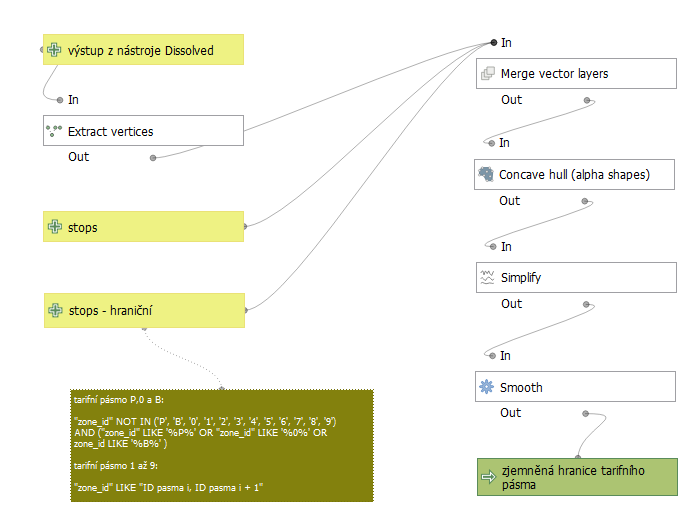
\includegraphics[width=400pt]{./pictures/postup-smooth.png}
    \caption[Postup pro zjemnění tvaru tarfních pásem]{Postup pro zjemnění tvaru tarfních pásem}
	\label{fig:postup-smooth}              
\end{figure}